%! Author = user
%! Date = 3/9/2024

% Preamble
\documentclass{article}
\usepackage[utf8]{inputenc}
\usepackage{amsmath, amssymb, amsthm}
\usepackage{tikz}
\usepackage{pgfplots}
\usepackage{listings}
\usepackage[labelformat=empty]{caption}
\usepackage[fontsize=13.5pt]{fontsize}
\usepackage[a4paper,
            bindingoffset=.2in,
            left=.7in,
            right=.7in,
            top=1in,
            bottom=1in,
            footskip=.25in]{geometry}

\definecolor{dkgreen}{rgb}{0,0.6,0}
\definecolor{gray}{rgb}{0.5,0.5,0.5}
\definecolor{mauve}{rgb}{0.58,0,0.82}

\lstset{frame=tb,
  language=Java,
  aboveskip=3mm,
  belowskip=3mm,
  showstringspaces=false,
  columns=flexible,
  basicstyle={\small\ttfamily},
  numbers=none,
  numberstyle=\tiny\color{gray},
  keywordstyle=\color{blue},
  commentstyle=\color{dkgreen},
  stringstyle=\color{mauve},
  breaklines=true,
  breakatwhitespace=true,
  tabsize=3
}

\title{LaTex for Students}
\author{Jun Ho Lee}
\date{April 2024}

% Document
\begin{document}

\newpage
\section{Week1}

Improving Deep Neural Network

\subsection{Setting up your ML application}

Train/dev/test sets

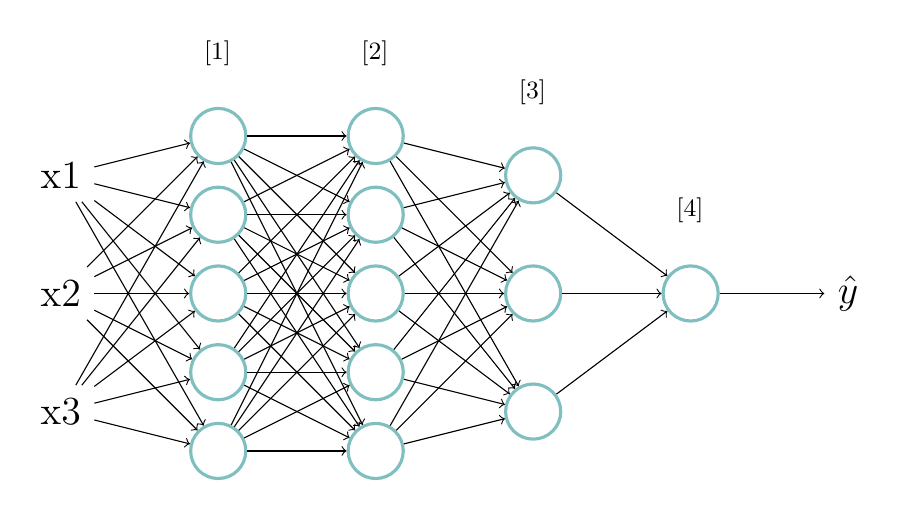
\begin{tikzpicture}
% Input Layer
\foreach \name/\i in {x1/1,x2/2,x3/3} {
    \node (Input-\i) at (0,-\i*1.5) {\name};
    \ifnum \i=1
        \node[above of=Input-\i] {};
    \fi
}
% Hidden Layer
\foreach \i in {1,2,3,4,5} {
    \node[circle, minimum size = 7mm, draw=teal!50, line width=.4mm]
    (Hidden1-\i) at (2,-\i) {};
    \ifnum \i=1
    \node[above of=Hidden1-\i] {$^{[1]}$};
    \fi
}
\foreach \i in {1,2,3,4,5} {
    \node[circle, minimum size = 7mm, draw=teal!50, line width=.4mm]
    (Hidden2-\i) at (4,-\i) {};
    \ifnum \i=1
    \node[above of=Hidden2-\i] {$^{[2]}$};
    \fi
}
\foreach \i in {1,2,3} {
    \node[circle, minimum size = 7mm, draw=teal!50, line width=.4mm]
    (Hidden3-\i) at (6,-\i*1.5) {};
    \ifnum \i=1
    \node[above of=Hidden3-\i] {$^{[3]}$};
    \fi
}
\foreach \i in {1} {
    \node[circle, minimum size = 7mm, draw=teal!50, line width=.4mm]
    (Hidden4-\i) at (8,-3) {};
    \ifnum \i=1
    \node[above of=Hidden4-\i] {$^{[4]}$};
    \fi
}
% Output Layer
\foreach \name/\i in {$\hat{y}$/1} {
    \node (Output-\i) at (10,-3) {\name};
    \ifnum \i=1
    \node[above of=Output-\i] {};
    \fi
}
% Arrows
\foreach \i in {1,2,3} {
    \foreach \j in {1,2,3,4,5} {
    \draw[->] (Input-\i) -- (Hidden1-\j);
    }
}
\foreach \i in {1,2,3,4,5} {
    \foreach \j in {1,2,3,4,5} {
    \draw[->] (Hidden1-\i) -- (Hidden2-\j);
    }
}
\foreach \i in {1,2,3,4,5} {
    \foreach \j in {1,2,3} {
    \draw[->] (Hidden2-\i) -- (Hidden3-\j);
    }
}
\foreach \i in {1,2,3} {
    \foreach \j in {1} {
    \draw[->] (Hidden3-\i) -- (Hidden4-\j);
    }
}
\foreach \i in {1} {
    \foreach \j in {1} { \draw[->] (Hidden4-\i) -- (Output-\j);
    }
}
\end{tikzpicture}\\

$Z^{[1]} = W^{[1]} A^{[0]} + b^{[1]} _{\hspace{5mm} where \hspace{1mm} A^{[0]} = X}$\\

$A^{[1]} = g^{[{1}]} (Z^{[1]})$\\

$Z^{[2]} = W^{[2]} A^{[1]} + b^{[2]}$\\

$A^{[2]} = g^{[{2}]} (Z^{[2]})$\\

\dots \\

$Z^{[4]} = W^{[4]} A^{[3]} + b^{[4]}$\\

$A^{[4]} = g^{[{4}]} (Z^{[4]}) = \hat{Y}$\\

\noindent\rule{8cm}{0.4pt}

Using for loops on $[l]$ layer for $l=1,2,\dots, L$:\\

$Z^{[l]} = W^{[l]} A^{[l-1]} + b^{[l]}$\\

$A^{[l]} = g^{[{l}]} (Z^{[l]})$\\


\newpage
\subsection{Forward and Backward Propagation}


$\indent$ Forward propagation for layer $l$: $a^{[l-1]}\rightarrow a^{[l]}, z^{[l]}, w^{[l]}, b^{[l]}$\\

$Z^{[l]} = W^{[l]} A^{[l-1]} + b^{[l]}$\\

$A^{[l]} = g^{[l]} (Z^{[l]})$\\

(for $i=1,\dots,L$ with initial value $A^{[0]} = X$)\\

Backward propagation for layer $l$: $da^{[l]} \rightarrow da^{[l-1]},dW^{[l]}, db^{[l]}$\\

$dZ^{[l]} = dA^{[l]} * {g^{[l]}}^{'}(Z^{[l]})$\\

$dW^{[l]} = \frac{1}{m}dZ^{[l]}{A^{[l-1]}}^T$\\

$db^{[l]} = \frac{1}{m}np.sum(dZ^{[l]}, axis=1, keepdims=True)$\\

$dA^{[l-1]} = {W^{[l]}}^T dZ^{[l]} = \frac{dJ}{dA^{[l-1]}} = \frac{dZ^{[l]}}{dA^{[l-1]}} \frac{dJ}{dZ^{[l]}} = \frac{dZ^{[l]}}{dA^{[l-1]}} dZ^{[l]}$\\

(with initial value $dZ^{[L]} = A^{[L]}-Y$)\\



\end{document}

